
\subsubsection{Analisi Derivazioni e Ridondanze}
In questa fase viene analizzata la struttura dello schema dal punto di vista delle ridondanze, della loro possibile esclusione e della possibilità di introdurne alcune in modo da ridurre il numero di accessi delle operazioni. \newline
Per quanto riguarda l'esclusione delle ridondanze, la strategia di progettazione è stata molto improntata sulla limitazione delle ridondaze e ciò ha portato alla presenza di un solo attributo che ha necessitato di un'attenta analisi. In questo caso ci riferiamo all'attributo Importo presente sia in Fattura che in Contratto di Assistenza on Center. La sua trattazione ha richiesto non poche analisi prima di realizzare che esso non è assimilabile ad una ridondanza. Importo nell'entità Fattura è vincolato dalla decisione di non conservare tutti i cataloghi dei fornitori. Quindi aggiornando mensilmente i prezzi dei cataloghi si perde la possibilità di andare a cercare il prezzo di un prodotto in un certo arco temporale se non quello attuale, e questo renderebbe impossibile calcolare l'importo di una fattura a posteriori.\newline
Questo implica che la presenza o l'assenza di questo attributo nella Fattura non porta allo stesso risultato, dal punto di vista logico, perciò esso non può essere considerato una ridondanza. Sarebbe altrettanto sbagliato considerare l'attributo ridondante quello nel Contratto di Assistenza in quanto esso è logicamente introdotto in un momento precedente alla creazione della fattura, e non il contrario.\newline\newline
Quindi si è concluso che non sono presenti ridondanze eliminabili, si è pensato allora all'introduzione di una ridondanza che potrebbe essere utile nel ridurre il numero di accessi al database, nel caso di operazioni di tipo statistico. Parliamo dell'aggiunta degli attributi Peso e Dimensioni (operazioni 6, 8, 13, 41) al Catalogo.
Consideriamo il caso della vendita di un prodotto che prevede, nella creazione della fattura, alcune operazioni necessarie per il calcolo dei costi di spedizione, che prendono in causa proprio questi parametri.
\noindent\newline
- 6 inserimento nuova fattura\newline
- 8 inserimento nuovo prodotto in catalogo\newline
- 13 aggiornamento prodotto in catalogo\newline
- 41 calcolo costi di spedizione
\newline\newline
Assumiamo un numero di prodotti pari a 3 all'interno della vendita.
\vspace{1cm}

\centerline{\textbf{ATTRIBUTO PESO IN CATALOGO}}
\vspace{1cm}
\centerline{\textbf{CON RIDONDANZA}}



\begin{table}[H]
\centering
\caption{Operazione 6}
\begin{tabular}{llll}
\\ \hline
\multicolumn{1}{|l|}{\textbf{CONCETTO}} & \multicolumn{1}{l|}{\textbf{COSTRUTTO}} & \multicolumn{1}{l|}{\textbf{ACCESSI}} & \multicolumn{1}{l|}{\textbf{TIPO}} \\ \hline
\multicolumn{1}{|l|}{Stipulazione Vendita}
& \multicolumn{1}{l|}{R}                  & \multicolumn{1}{l|}{3}                & \multicolumn{1}{l|}{S}             \\ \hline
\multicolumn{1}{|l|}{Catalogo}             & \multicolumn{1}{l|}{R}                  & \multicolumn{1}{l|}{3}
& \multicolumn{1}{l|}{L}
			 \\ \hline
\multicolumn{1}{|l|}{Costo di Spedizione}     & \multicolumn{1}{l|}{E}                  & \multicolumn{1}{l|}{3}      & \multicolumn{1}{l|}{L}
			 \\ \hline
\multicolumn{1}{|l|}{Fattura}
& \multicolumn{1}{l|}{E}                  & \multicolumn{1}{l|}{1}                & \multicolumn{1}{l|}{S}             \\ \hline
\end{tabular}
\end{table}

\begin{table}[H]
\centering
\caption{Operazione 8}
\begin{tabular}{llll}
\\ \hline
\multicolumn{1}{|l|}{\textbf{CONCETTO}} & \multicolumn{1}{l|}{\textbf{COSTRUTTO}} & \multicolumn{1}{l|}{\textbf{ACCESSI}} & \multicolumn{1}{l|}{\textbf{TIPO}} \\ \hline
\multicolumn{1}{|l|}{Catalogo}
& \multicolumn{1}{l|}{R}                  & \multicolumn{1}{l|}{1}                & \multicolumn{1}{l|}{S}             \\ \hline
\end{tabular}
\end{table}

\begin{table}[H]
\centering
\caption{Operazione 13}
\begin{tabular}{llll}
\\ \hline
\multicolumn{1}{|l|}{\textbf{CONCETTO}} & \multicolumn{1}{l|}{\textbf{COSTRUTTO}} & \multicolumn{1}{l|}{\textbf{ACCESSI}} & \multicolumn{1}{l|}{\textbf{TIPO}} \\ \hline
\multicolumn{1}{|l|}{Catalogo}
& \multicolumn{1}{l|}{R}                  & \multicolumn{1}{l|}{1}                & \multicolumn{1}{l|}{S}             \\ \hline
\end{tabular}
\end{table}


\begin{table}[H]
\centering
\caption{Operazione 41}
\begin{tabular}{llll}
\\ \hline
\multicolumn{1}{|l|}{\textbf{CONCETTO}} & \multicolumn{1}{l|}{\textbf{COSTRUTTO}} & \multicolumn{1}{l|}{\textbf{ACCESSI}} & \multicolumn{1}{l|}{\textbf{TIPO}} \\ \hline
\multicolumn{1}{|l|}{Catalogo}
& \multicolumn{1}{l|}{R}                  & \multicolumn{1}{l|}{1}                & \multicolumn{1}{l|}{L}             \\ \hline
\multicolumn{1}{|l|}{Spedizione}
& \multicolumn{1}{l|}{R}                  & \multicolumn{1}{l|}{1}                & \multicolumn{1}{l|}{L}             \\ \hline
\end{tabular}
\end{table}

\vspace{1cm}
\centerline{\textbf{SENZA RIDONDANZA}}

\begin{table}[H]
\centering
\caption{Operazione 6}
\begin{tabular}{llll}
\\ \hline
\multicolumn{1}{|l|}{\textbf{CONCETTO}} & \multicolumn{1}{l|}{\textbf{COSTRUTTO}} & \multicolumn{1}{l|}{\textbf{ACCESSI}} & \multicolumn{1}{l|}{\textbf{TIPO}} \\ \hline
\multicolumn{1}{|l|}{Stipulazione Vendita}
& \multicolumn{1}{l|}{R}                  & \multicolumn{1}{l|}{3}                & \multicolumn{1}{l|}{S}             \\ \hline
\multicolumn{1}{|l|}{Catalogo}             & \multicolumn{1}{l|}{R}                  & \multicolumn{1}{l|}{3}
& \multicolumn{1}{l|}{L}
			 \\ \hline
\multicolumn{1}{|l|}{Prodotto}             & \multicolumn{1}{l|}{E}                  & \multicolumn{1}{l|}{3}
& \multicolumn{1}{l|}{L}
			 \\ \hline
\multicolumn{1}{|l|}{Costo di Spedizione}     & \multicolumn{1}{l|}{E}                  & \multicolumn{1}{l|}{3}      & \multicolumn{1}{l|}{L}
			 \\ \hline
\multicolumn{1}{|l|}{Fattura}
& \multicolumn{1}{l|}{E}                  & \multicolumn{1}{l|}{1}                & \multicolumn{1}{l|}{S}             \\ \hline
\end{tabular}
\end{table}

\begin{table}[H]
\centering
\caption{Operazione 8}
\begin{tabular}{llll}
\\ \hline
\multicolumn{1}{|l|}{\textbf{CONCETTO}} & \multicolumn{1}{l|}{\textbf{COSTRUTTO}} & \multicolumn{1}{l|}{\textbf{ACCESSI}} & \multicolumn{1}{l|}{\textbf{TIPO}} \\ \hline
\multicolumn{1}{|l|}{Catalogo}
& \multicolumn{1}{l|}{R}                  & \multicolumn{1}{l|}{1}                & \multicolumn{1}{l|}{S}             \\ \hline
\end{tabular}
\end{table}

\begin{table}[H]
\centering
\caption{Operazione 13}
\begin{tabular}{llll}
\\ \hline
\multicolumn{1}{|l|}{\textbf{CONCETTO}} & \multicolumn{1}{l|}{\textbf{COSTRUTTO}} & \multicolumn{1}{l|}{\textbf{ACCESSI}} & \multicolumn{1}{l|}{\textbf{TIPO}} \\ \hline
\multicolumn{1}{|l|}{Catalogo}
& \multicolumn{1}{l|}{R}                  & \multicolumn{1}{l|}{1}                & \multicolumn{1}{l|}{S}             \\ \hline
\end{tabular}
\end{table}


\begin{table}[H]
\centering
\caption{Operazione 41}
\begin{tabular}{llll}
\\ \hline
\multicolumn{1}{|l|}{\textbf{CONCETTO}} & \multicolumn{1}{l|}{\textbf{COSTRUTTO}} & \multicolumn{1}{l|}{\textbf{ACCESSI}} & \multicolumn{1}{l|}{\textbf{TIPO}} \\ \hline
\multicolumn{1}{|l|}{Prodotto}             & \multicolumn{1}{l|}{E}                  & \multicolumn{1}{l|}{1}
& \multicolumn{1}{l|}{L}
			 \\ \hline
\multicolumn{1}{|l|}{Spedizione}
& \multicolumn{1}{l|}{R}                  & \multicolumn{1}{l|}{1}                & \multicolumn{1}{l|}{L}             \\ \hline
\end{tabular}
\end{table}


\begin{table}[H]
\centering
\caption{Costo Operazioni con ridondanza}
\label{my-label}
\resizebox{\textwidth}{!}{%
\begin{tabular}{|l|l|l|l|}
\hline
\textbf{OPERAZIONE}               & \textbf{COSTO} & \textbf{FREQUENZA} & \textbf{TOTALE} \\ \hline
6                                & 10             & 69              & 690
\\ \hline
8                                & 1              & 0.1667          & 0.1667
\\ \hline
13                                & 1              & 10             & 10
\\ \hline
41                                & 2              & 69             & 138
\\ \hline
COSTO OPERAZIONI CON RIDONDANZA & 14        &                    &   \hl{838.1667}             \\ \hline
\end{tabular}
}
\end{table}


\begin{table}[H]
\centering
\caption{Costo Operazioni senza ridondanza}
\label{my-label}
\resizebox{\textwidth}{!}{%
\begin{tabular}{|l|l|l|l|}
\hline
\textbf{OPERAZIONE}             & \textbf{COSTO} & \textbf{FREQUENZA} & \textbf{TOTALE} \\ \hline
6                                & 13             & 69             & 897
\\ \hline
8                                & 1              & 0.1667		   & 0.1667
\\ \hline
13                                & 1              & 10            & 10
\\ \hline
41                                & 2              & 69            & 138
\\ \hline
COSTO OPERAZIONI SENZA RIDONDANZA & 17        &                    &  \hl{1045.1667}          \\ \hline
\end{tabular}
}
\end{table}

\vspace{1.5cm}
Per l'attributo Dimensioni si ha esattamente la stessa situazione
\vspace{1cm}

\centerline{\textbf{ATTRIBUTO DIMENSIONI IN CATALOGO}}
\vspace{1cm}
\centerline{\textbf{CON RIDONDANZA}}

\begin{table}[H]
\centering
\caption{Operazione 6}
\begin{tabular}{llll}
\\ \hline
\multicolumn{1}{|l|}{\textbf{CONCETTO}} & \multicolumn{1}{l|}{\textbf{COSTRUTTO}} & \multicolumn{1}{l|}{\textbf{ACCESSI}} & \multicolumn{1}{l|}{\textbf{TIPO}} \\ \hline
\multicolumn{1}{|l|}{Stipulazione Vendita}
& \multicolumn{1}{l|}{R}                  & \multicolumn{1}{l|}{3}                & \multicolumn{1}{l|}{S}             \\ \hline
\multicolumn{1}{|l|}{Catalogo}             & \multicolumn{1}{l|}{R}                  & \multicolumn{1}{l|}{3}
& \multicolumn{1}{l|}{L}
			 \\ \hline
\multicolumn{1}{|l|}{Costo di Spedizione}     & \multicolumn{1}{l|}{E}                  & \multicolumn{1}{l|}{3}      & \multicolumn{1}{l|}{L}
			 \\ \hline
\multicolumn{1}{|l|}{Fattura}
& \multicolumn{1}{l|}{E}                  & \multicolumn{1}{l|}{1}                & \multicolumn{1}{l|}{S}             \\ \hline
\end{tabular}
\end{table}

\begin{table}[H]
\centering
\caption{Operazione 8}
\begin{tabular}{llll}
\\ \hline
\multicolumn{1}{|l|}{\textbf{CONCETTO}} & \multicolumn{1}{l|}{\textbf{COSTRUTTO}} & \multicolumn{1}{l|}{\textbf{ACCESSI}} & \multicolumn{1}{l|}{\textbf{TIPO}} \\ \hline
\multicolumn{1}{|l|}{Catalogo}
& \multicolumn{1}{l|}{R}                  & \multicolumn{1}{l|}{1}                & \multicolumn{1}{l|}{S}             \\ \hline
\end{tabular}
\end{table}

\begin{table}[H]
\centering
\caption{Operazione 13}
\begin{tabular}{llll}
\\ \hline
\multicolumn{1}{|l|}{\textbf{CONCETTO}} & \multicolumn{1}{l|}{\textbf{COSTRUTTO}} & \multicolumn{1}{l|}{\textbf{ACCESSI}} & \multicolumn{1}{l|}{\textbf{TIPO}} \\ \hline
\multicolumn{1}{|l|}{Catalogo}
& \multicolumn{1}{l|}{R}                  & \multicolumn{1}{l|}{1}                & \multicolumn{1}{l|}{S}             \\ \hline
\end{tabular}
\end{table}


\begin{table}[H]
\centering
\caption{Operazione 41}
\begin{tabular}{llll}
\\ \hline
\multicolumn{1}{|l|}{\textbf{CONCETTO}} & \multicolumn{1}{l|}{\textbf{COSTRUTTO}} & \multicolumn{1}{l|}{\textbf{ACCESSI}} & \multicolumn{1}{l|}{\textbf{TIPO}} \\ \hline
\multicolumn{1}{|l|}{Catalogo}
& \multicolumn{1}{l|}{R}                  & \multicolumn{1}{l|}{1}                & \multicolumn{1}{l|}{L}             \\ \hline
\multicolumn{1}{|l|}{Spedizione}
& \multicolumn{1}{l|}{R}                  & \multicolumn{1}{l|}{1}                & \multicolumn{1}{l|}{L}             \\ \hline
\end{tabular}
\end{table}

\vspace{1cm}
\centerline{\textbf{SENZA RIDONDANZA}}

\begin{table}[H]
\centering
\caption{Operazione 6}
\begin{tabular}{llll}
\\ \hline
\multicolumn{1}{|l|}{\textbf{CONCETTO}} & \multicolumn{1}{l|}{\textbf{COSTRUTTO}} & \multicolumn{1}{l|}{\textbf{ACCESSI}} & \multicolumn{1}{l|}{\textbf{TIPO}} \\ \hline
\multicolumn{1}{|l|}{Stipulazione Vendita}
& \multicolumn{1}{l|}{R}                  & \multicolumn{1}{l|}{3}                & \multicolumn{1}{l|}{S}             \\ \hline
\multicolumn{1}{|l|}{Catalogo}             & \multicolumn{1}{l|}{R}                  & \multicolumn{1}{l|}{3}
& \multicolumn{1}{l|}{L}
			 \\ \hline
\multicolumn{1}{|l|}{Prodotto}             & \multicolumn{1}{l|}{E}                  & \multicolumn{1}{l|}{3}
& \multicolumn{1}{l|}{L}
			 \\ \hline
\multicolumn{1}{|l|}{Costo di Spedizione}     & \multicolumn{1}{l|}{E}                  & \multicolumn{1}{l|}{3}      & \multicolumn{1}{l|}{L}
			 \\ \hline
\multicolumn{1}{|l|}{Fattura}
& \multicolumn{1}{l|}{E}                  & \multicolumn{1}{l|}{1}                & \multicolumn{1}{l|}{S}             \\ \hline
\end{tabular}
\end{table}

\begin{table}[H]
\centering
\caption{Operazione 8}
\begin{tabular}{llll}
\\ \hline
\multicolumn{1}{|l|}{\textbf{CONCETTO}} & \multicolumn{1}{l|}{\textbf{COSTRUTTO}} & \multicolumn{1}{l|}{\textbf{ACCESSI}} & \multicolumn{1}{l|}{\textbf{TIPO}} \\ \hline
\multicolumn{1}{|l|}{Catalogo}
& \multicolumn{1}{l|}{R}                  & \multicolumn{1}{l|}{1}                & \multicolumn{1}{l|}{S}             \\ \hline
\end{tabular}
\end{table}

\begin{table}[H]
\centering
\caption{Operazione 13}
\begin{tabular}{llll}
\\ \hline
\multicolumn{1}{|l|}{\textbf{CONCETTO}} & \multicolumn{1}{l|}{\textbf{COSTRUTTO}} & \multicolumn{1}{l|}{\textbf{ACCESSI}} & \multicolumn{1}{l|}{\textbf{TIPO}} \\ \hline
\multicolumn{1}{|l|}{Catalogo}
& \multicolumn{1}{l|}{R}                  & \multicolumn{1}{l|}{1}                & \multicolumn{1}{l|}{S}             \\ \hline
\end{tabular}
\end{table}


\begin{table}[H]
\centering
\caption{Operazione 41}
\begin{tabular}{llll}
\\ \hline
\multicolumn{1}{|l|}{\textbf{CONCETTO}} & \multicolumn{1}{l|}{\textbf{COSTRUTTO}} & \multicolumn{1}{l|}{\textbf{ACCESSI}} & \multicolumn{1}{l|}{\textbf{TIPO}} \\ \hline
\multicolumn{1}{|l|}{Prodotto}             & \multicolumn{1}{l|}{E}                  & \multicolumn{1}{l|}{1}
& \multicolumn{1}{l|}{L}
			 \\ \hline
\multicolumn{1}{|l|}{Spedizione}
& \multicolumn{1}{l|}{R}                  & \multicolumn{1}{l|}{1}                & \multicolumn{1}{l|}{L}             \\ \hline
\end{tabular}
\end{table}


\begin{table}[H]
\centering
\caption{Costo Operazioni con ridondanza}
\label{my-label}
\resizebox{\textwidth}{!}{%
\begin{tabular}{|l|l|l|l|}
\hline
\textbf{OPERAZIONE}               & \textbf{COSTO} & \textbf{FREQUENZA} & \textbf{TOTALE} \\ \hline
6                                & 10             & 69              & 690
\\ \hline
8                                & 1              & 0.1667          & 0.1667
\\ \hline
13                                & 1              & 10             & 10
\\ \hline
41                                & 2              & 69             & 138
\\ \hline
COSTO OPERAZIONI CON RIDONDANZA & 14        &                    &   \hl{838.1667}             \\ \hline
\end{tabular}
}
\end{table}


\begin{table}[H]
\centering
\caption{Costo Operazioni senza ridondanza}
\label{my-label}
\resizebox{\textwidth}{!}{%
\begin{tabular}{|l|l|l|l|}
\hline
\textbf{OPERAZIONE}             & \textbf{COSTO} & \textbf{FREQUENZA} & \textbf{TOTALE} \\ \hline
6                                & 13             & 69             & 897
\\ \hline
8                                & 1              & 0.1667		   & 0.1667
\\ \hline
13                                & 1              & 10            & 10
\\ \hline
41                                & 2              & 69            & 138
\\ \hline
COSTO OPERAZIONI SENZA RIDONDANZA & 17        &                    &  \hl{1045.1667}          \\ \hline
\end{tabular}
}
\end{table}

\vspace{1cm}
\noindent
Quanto risulta da entrambe le analisi, che sono in realtà la stessa per i due attributi, risulta che il guadagno portato dalla presenza dell'attributo ridondante su catalogo non è particolarmente decisivo sul numero di operazioni che vengono eseguite, infatti non vengono nemmeno dimezzate il numero di operazioni. Con questi risultati si è preferito evitare l'introduzione delle ridondanze nella relazione Catalogo, favorendo, anche se di poco, l'aspetto spaziale, mantenendo quindi lo schema inalterato.


\newpage
\subsubsection{Eliminazione Delle Gerarchie}

Nel nostro schema concettuale sono presenti 5 generalizzazioni. Le Entità coinvolte sono "PA, Azienda o Persona", "Cliente", "Richiesta sul Mepa", "Prodotto o servizio", "Prodotto".
\newline
Abbiamo deciso di procedere nel seguente modo:

\paragraph{PA, Azienda o Persona}
Per quanto riguarda l'entità PA, Azienda o Persona, abbiamo scelto di accorpare il genitore della generalizzazione nelle entità figlie. Questo perchè i clienti e i fornitori hanno rapporti con l'azienda piuttosto diversi tra loro, quindi la separazione comporta una suddivisione concettuale che migliora la chiarezza dello schema.
\paragraph{Cliente}
Per l'entità Cliente si è adottata una soluzione ibrida. Abbiamo optato per mantenere l'entità figlia Pubblica Amministrazione, mentre l'entità Privato è stata accorpata nel genitore aggiungendo un nuovo attributo "Tipo", che indica appunto se il Cliente è un Privato o una PA. Un eventuale accorpamento del genitore nelle entità figlie avrebbe complicato lo schema, viste le numerose relazioni che ha il genitore.
\newline
La relazione tra Cliente e PA è denominata "Specificazione PA".
\paragraph{Richiesta sul Mepa}
In merito all'entità Richiesta sul Mepa, si è deciso di sostituire la generalizzazione con delle relazioni. Avremmo potuto accorpare le entità figlie nel genitore, utilizzando degli attributi che possono assumere il valore NULL per poter distinguire appunto le due entità, ma ci sembra più opportuno mantenere distinte le entità Gara pubblica e Trattativa diretta in quanto esse sono, nella realtà pratica, due concetti logicamente separati.
Le nuove relazioni sono denominate "Specificazione gara" e "Specificazione trattativa".
\paragraph{Prodotto o Servizio}
Anche con l'entità Prodotto o Servizio abbiamo scelto di mantenere il genitore e le entità figlie, sostituendo la generalizzazione con delle relazioni. Le nuove relazioni sono "Specificazione prodotto" e "Specificazione Servizio".
\paragraph{Prodotto}
Per l'entità Prodotto si è scelto di mantenere sia il padre che le entità figlie, dato che queste ultime hanno tanti attributi diversi, e l'accorpamento nell'entità genitore significherebbe avere tanti valori con valore NULL. Inoltre, un eventuale accorpamento del genitore nelle entità figlie risulterebbe piuttosto complicato, date le numerose relazioni che ha il padre e visto che le entità figlie sono molteplici.
Quindi, si è scelto di sostituire la generalizzazione con delle relazioni, una per ogni entità figlia. Le nuove relazioni sono denominate "Specificazione" più il nome dell'entità a cui si riferiscono.
\newline\newline
In seguito all'aggiunta dell'attributo "Tipo" all'entità "Cliente", è necessario introdurre una nuova regola di vincolo:

\begin{itemize}
  \item L'attributo "Tipo" relativo all'entità "Cliente" può essere "Privato" oppure "PA".
\end{itemize}
\noindent
\textit{(Facciamo notare che, per non appesantire ulteriormente lo schema, abbiamo scelto di togliere alcuni prodotti e di mantenere solo "Notebook", "Pc Desktop", "Monitor", "Stampante")}



\newpage
\begin{landscape} %inizia un foglio landscape

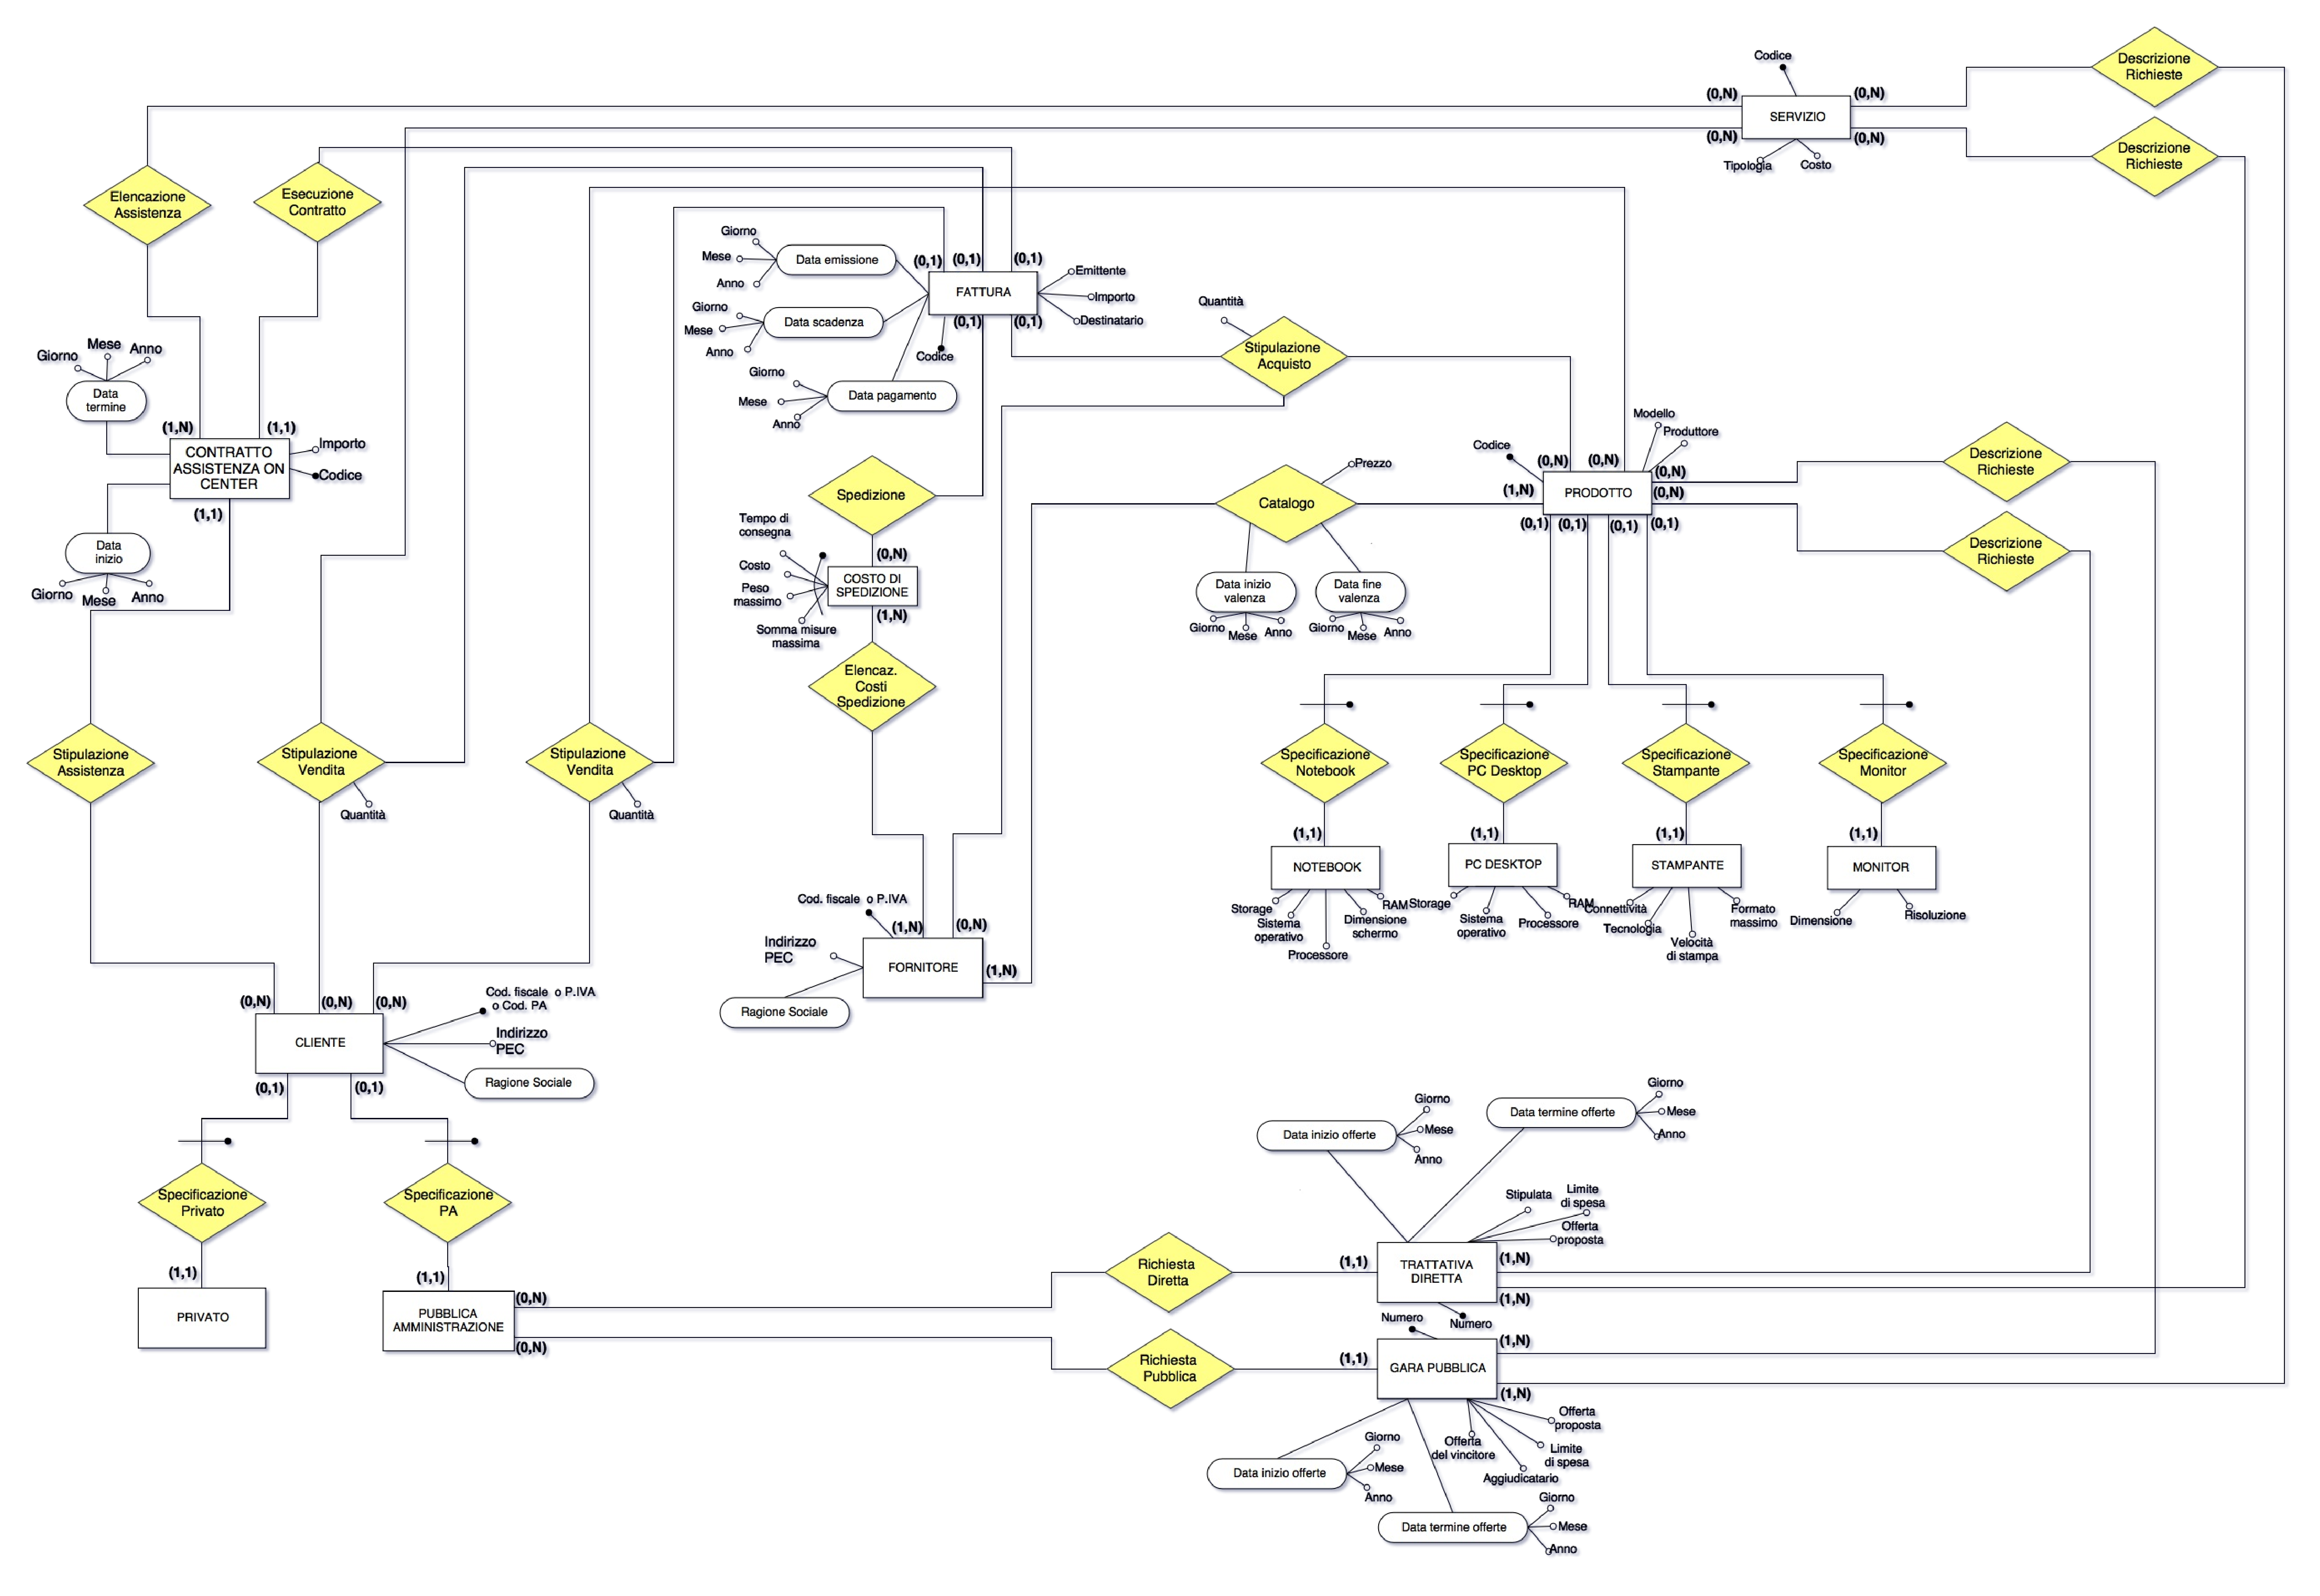
\includepdf[angle=90]{./immagini/modello_er_v3.pdf}

\end{landscape}


\newpage
\subsubsection{Eliminazione degli Attributi Multivalore}

Abbiamo individuato un solo attributo multivalore, l'attributo Telefono nelle entità Cliente e Fornitore, in quanto abbiamo ritenuto che sia possibile che una di queste entità possa avere più numeri di telefono associati.
\newline
Relativamente alle relazioni qui sopra citate abbiamo eseguito la ristrutturazione seguente:
\newline\newline

\noindent\makebox[\textwidth]{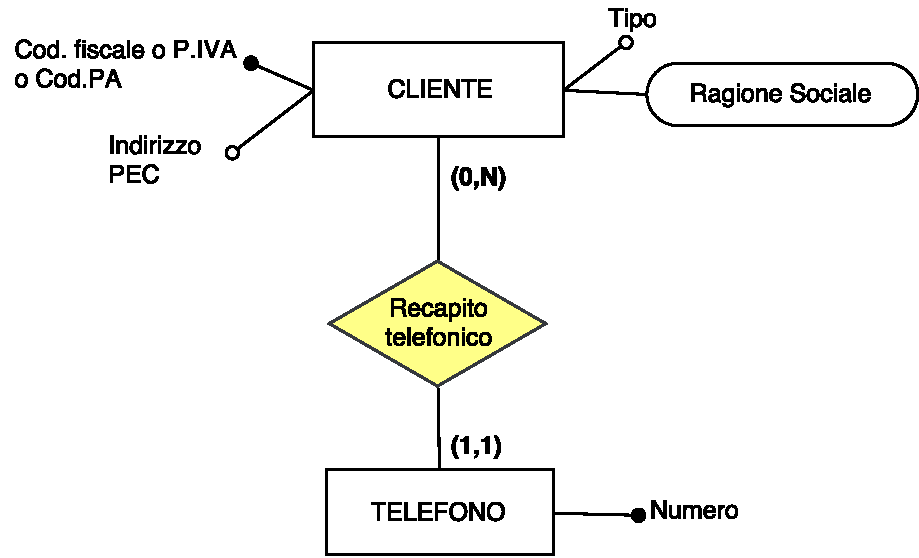
\includegraphics[width=0.7\linewidth]{./immagini/recapito_telefonico.pdf}}
\newline\newline
Tale ristrutturazione, relativa all'entità Cliente, è analoga a Fornitore, perciò non vengono riportate le modifiche a tale entità.
